
\section{Calculations \& Graphs}

\vspace{-0.5cm}
\singlespacing

%------- Force --------%

\subsection{Spring Constant of Spring} 

{\centering
\begin{equation}
	k =  \frac{-F}{x} 
	\label{eq:springK}
\end{equation}
\begin{align*}
	k &: \text{spring constant} \\
	\mathbf{F} &: \text{weight of hanging mass} \\
	x &: \text{equilibrium position}
\end{align*}}

\subsubsection{Sample Calculation \\ {\normalfont \small\textit{using average force of part 1}}}

{\centering
\begin{align*}
	k &=  \frac{-F}{x} \\ \\
		&=  \frac{2 \pi (0.2\text{ m})}{0.3426\text{ s}} \\ \\
	v	&= \boxed{3.666 \text{ m/s}} 
\end{align*}}

%------- ACCELERATION BETWEEN TWO POINTS WITH INITIAL VELOCITY CLOSE TO ZERO--------%

\subsection{Period of a Spring with A Hanging Mass} 

{\centering
\begin{equation}
	\text{T} = 2\pi \sqrt{\frac{m}{k}}
	\label{eq:springMass}
\end{equation}
\begin{align*}
	\text{T} &: \text{period} \\
	m &: \text{mass of hanging weight and spring} \\
	k &: \text{spring constant}
\end{align*}}

\subsubsection{Sample Calculation \\ {\normalfont \small\textit{part 1, mass of 50 g}}}

{\centering
\begin{align*}
	\text{T} &= 2\pi \sqrt{\frac{m}{k}} \\ \\
			&= \frac{(0.012\text{ kg})(2.858\text{ m/s})^2}{0.2\text{ m}} \\
	\text{F\textsubscript{c}}  &= \boxed{0.49\,\text{N}}
\end{align*}}

\subsection{Period of a Pendulum} 

{\centering
\begin{equation}
	\text{T} = 2\pi \sqrt{\frac{l}{g}}
	\label{eq:pendulum}
\end{equation}
\begin{align*}
	\text{T} &: \text{period} \\
	l &: \text{length of pendulum} \\
	g &: \text{acceleration due to gravity}
\end{align*}}

\subsubsection{Sample Calculation \\ {\normalfont \small\textit{part 1, mass of 50 g}}}

{\centering
\begin{align*}
	\text{T} &= 2\pi \sqrt{\frac{l}{g}} \\ \\
			&= \frac{(0.012\text{ kg})(2.858\text{ m/s})^2}{0.2\text{ m}} \\
	\text{F\textsubscript{c}}  &= \boxed{0.49\,\text{N}}
\end{align*}}

%------- ACCELERATION BETWEEN TWO POINTS --------%

%------- AVERAGE VALUE --------%


\subsection{Fractional Discrepancy}
\vspace{0.5cm}
\begin{equation}
	\text{FD}	= \left| \frac{\text{measured - actual}}{\text{actual}} \right|\
	\label{eq:fdisc}
\end{equation}

\subsubsection{Sample Calculation \\ {\normalfont \small\textit{percent error between theoretical period and measured period using values from part 3}}}

\begin{align*}
	\text{FD}	&= \left| \frac{\text{measured - actual}}{\text{actual}} \right|\ \\ \\
	\text{FD}	&= \left| \frac{\text{0.3426\text{ s} - 0.5071\text{ s}}}{\text{0.5071\text{ s}}} \right|\ \\ \\
			FD &= \boxed{32.41\%} 
\end{align*}
%------- AVERAGE VALUE --------%

%------- STANDARD DEVIATION --------%
%\subsection{Standard Deviation Formula}
%
%\begin{align*}
%		\sigma &= \sqrt{\frac{\Sigma(x_i -\overline{a})^2}{N}} \\
%		 &= \sqrt{\frac{SS}{N}} \\ \\
%		\textbf{N} &:\, \text{Total number of values} \\
%		\overline{\textbf{a}} &:\, \text{Average value} \\
%		\textbf{x\textsubscript{i}} &:\, \text{Each value from the data set} \\
%		\textbf{SS} &:\, \text{Sum of squares} 
%\end{align*}
%
%\subsubsection{Sample Calculation \\ {\normalfont \small\textit{std of photogate times with hanging mass at 10 grams }}}
%
%\begin{align*}
%	\sigma &= \sqrt{\frac{(1.461-\overline{a})^2 + ... + (1.454-\overline{a})^2}{3}} \\
%				 &= \sqrt{\frac{2.886\,\text{x}\,10^{-5}}{3}} \\
%		 &= \boxed{0.0003\, \text{s}}
%\end{align*}
%------- STANDARD DEVIATION --------%

%------- RELATIVE ERROR --------%
\subsection{Percent Error}
\vspace{0.5cm}
\begin{equation}
	\text{PD}	= \left| \frac{\text{measured - actual}}{\text{actual}} \right|\: \text{x}\: 100\%
	\label{eq:perror}
\end{equation}

\subsubsection{Sample Calculation \\ {\normalfont \small\textit{percent error between theoretical period and measured period using values from part 3}}}

\begin{align*}
	\text{PD}	&= \left| \frac{\text{measured - actual}}{\text{actual}} \right|\: \text{x}\: 100\% \\ \\
	\text{PD}	&= \left| \frac{\text{0.3426\text{ s} - 0.5071\text{ s}}}{\text{0.5071\text{ s}}} \right|\: \text{x}\: 100\% \\ \\
			PD &= \boxed{32.41\%} 
\end{align*}
%------- RELATIVE ERROR --------%

%----TABLES-----%
\subsection{Tables}

\begin{table}[H]
\centering
\captionsetup{font=Large}
\caption{Part 1 }
\resizebox{\columnwidth}{!}{%
\begin{tabular}{@{}ccccc@{}}
\toprule
\textbf{Mass (kg)}                       & 0.05   & 0.06  & 0.07  & 0.08   \\ \midrule
\textbf{Trial 1  Period (s)}             & 0.334  & 0.329 & 0.332 & 0.359  \\
\textbf{Trial 2 Period (s)}              & 0.3515 & 0.353 & 0.354 & 0.3295 \\
\textbf{Average Period (s)}              & 0.3427 & 0.341 & 0.343 & 0.3442 \\
\textbf{Average Velocity (m/s)}          & 3.666  & 3.685 & 3.663 & 3.65   \\
\textbf{Expected F\textsubscript{c} (N)} & 0.49   & 0.588 & 0.686 & 0.784  \\
\textbf{Actual F\textsubscript{c} (N)}   & 1.072  & 1.083 & 1.07  & 1.062  \\ \bottomrule
\end{tabular}%
}
\label{tab:part1Tab}
\end{table}

\begin{table}[H]
\centering
\captionsetup{font=Large}
\caption{Part 2}
\label{tab:part2Tab}
\resizebox{\columnwidth}{!}{%
\begin{tabular}{@{}ccccc@{}}
\toprule
\textbf{Mass (kg)}                       & 0.05   & 0.06   & 0.07   & 0.08   \\ \midrule
\textbf{Theoretical Velocity (m/s)}      & 2.478  & 2.715  & 2.932  & 3.135  \\
\textbf{Theoretical Period (s)}          & 0.5069 & 0.4627 & 0.4284 & 0.4007 \\
\textbf{Actual Period (from part 1) (s)} & 0.3427 & 0.341  & 0.343  & 0.3442 \\
\textbf{Percent Error}                   & 32.39  & 26.31  & 19.94  & 14.1   \\ \bottomrule
\end{tabular}%
}
\end{table}

\begin{table}[H]
\centering
\captionsetup{font=Large}
\caption{Part 3}
\label{tab:part3Tab}
\resizebox{\columnwidth}{!}{%
\begin{tabular}{@{}ccccc@{}}
\toprule
\textbf{Radius (m)}             & 0.1    & 0.15   & 0.2    & 0.3    \\ \midrule
\textbf{Trial 1  Period (s)}    & 0.273  & 0.7    & 0.5015 & 0.5625 \\
\textbf{Trial 2 Period (s)}     & 0.252  & 0.4575 & 0.5015 & 0.568  \\
\textbf{Average Period (s)}     & 0.2625 & 0.5787 & 0.5015 & 0.5652  \\
\textbf{Expected Velocity (m/s)} & 2.146  & 2.629  & 3.035  & 3.718 \\
\textbf{Average Velocity (m/s)} & 2.393  & 1.628  & 2.505  & 3.335 \\
\textbf{Percent Error Velocity (\%)} & 11.50  & 38.07  & 17.46  & 10.30 \\
\textbf{Expected F\textsubscript{c} (N)} & 0.735 & 0.735 & 0.735 & 0.735 \\ 
\textbf{Actual F\textsubscript{c} (N)} & 0.9133 & 0.2818 & 0.5004 & 0.5913 \\ 
\textbf{Percent Error F\textsubscript{c} (\%)} & 24.25  & 61.65  & 31.91  & 19.55 \\ \bottomrule
\end{tabular}%
}
\end{table}

\newpage
%----TABLES-----%

%----GRAPHS-----%
\subsection{Graphs}
% \begin{landscape}
% \subsection{Graphs}
% \begin{figure}[H]
% 	\begin{center}
% 		\captionsetup{font=Large}
% 		\caption{Force vs. Acceleration}\label{fig:GFvA}
% 		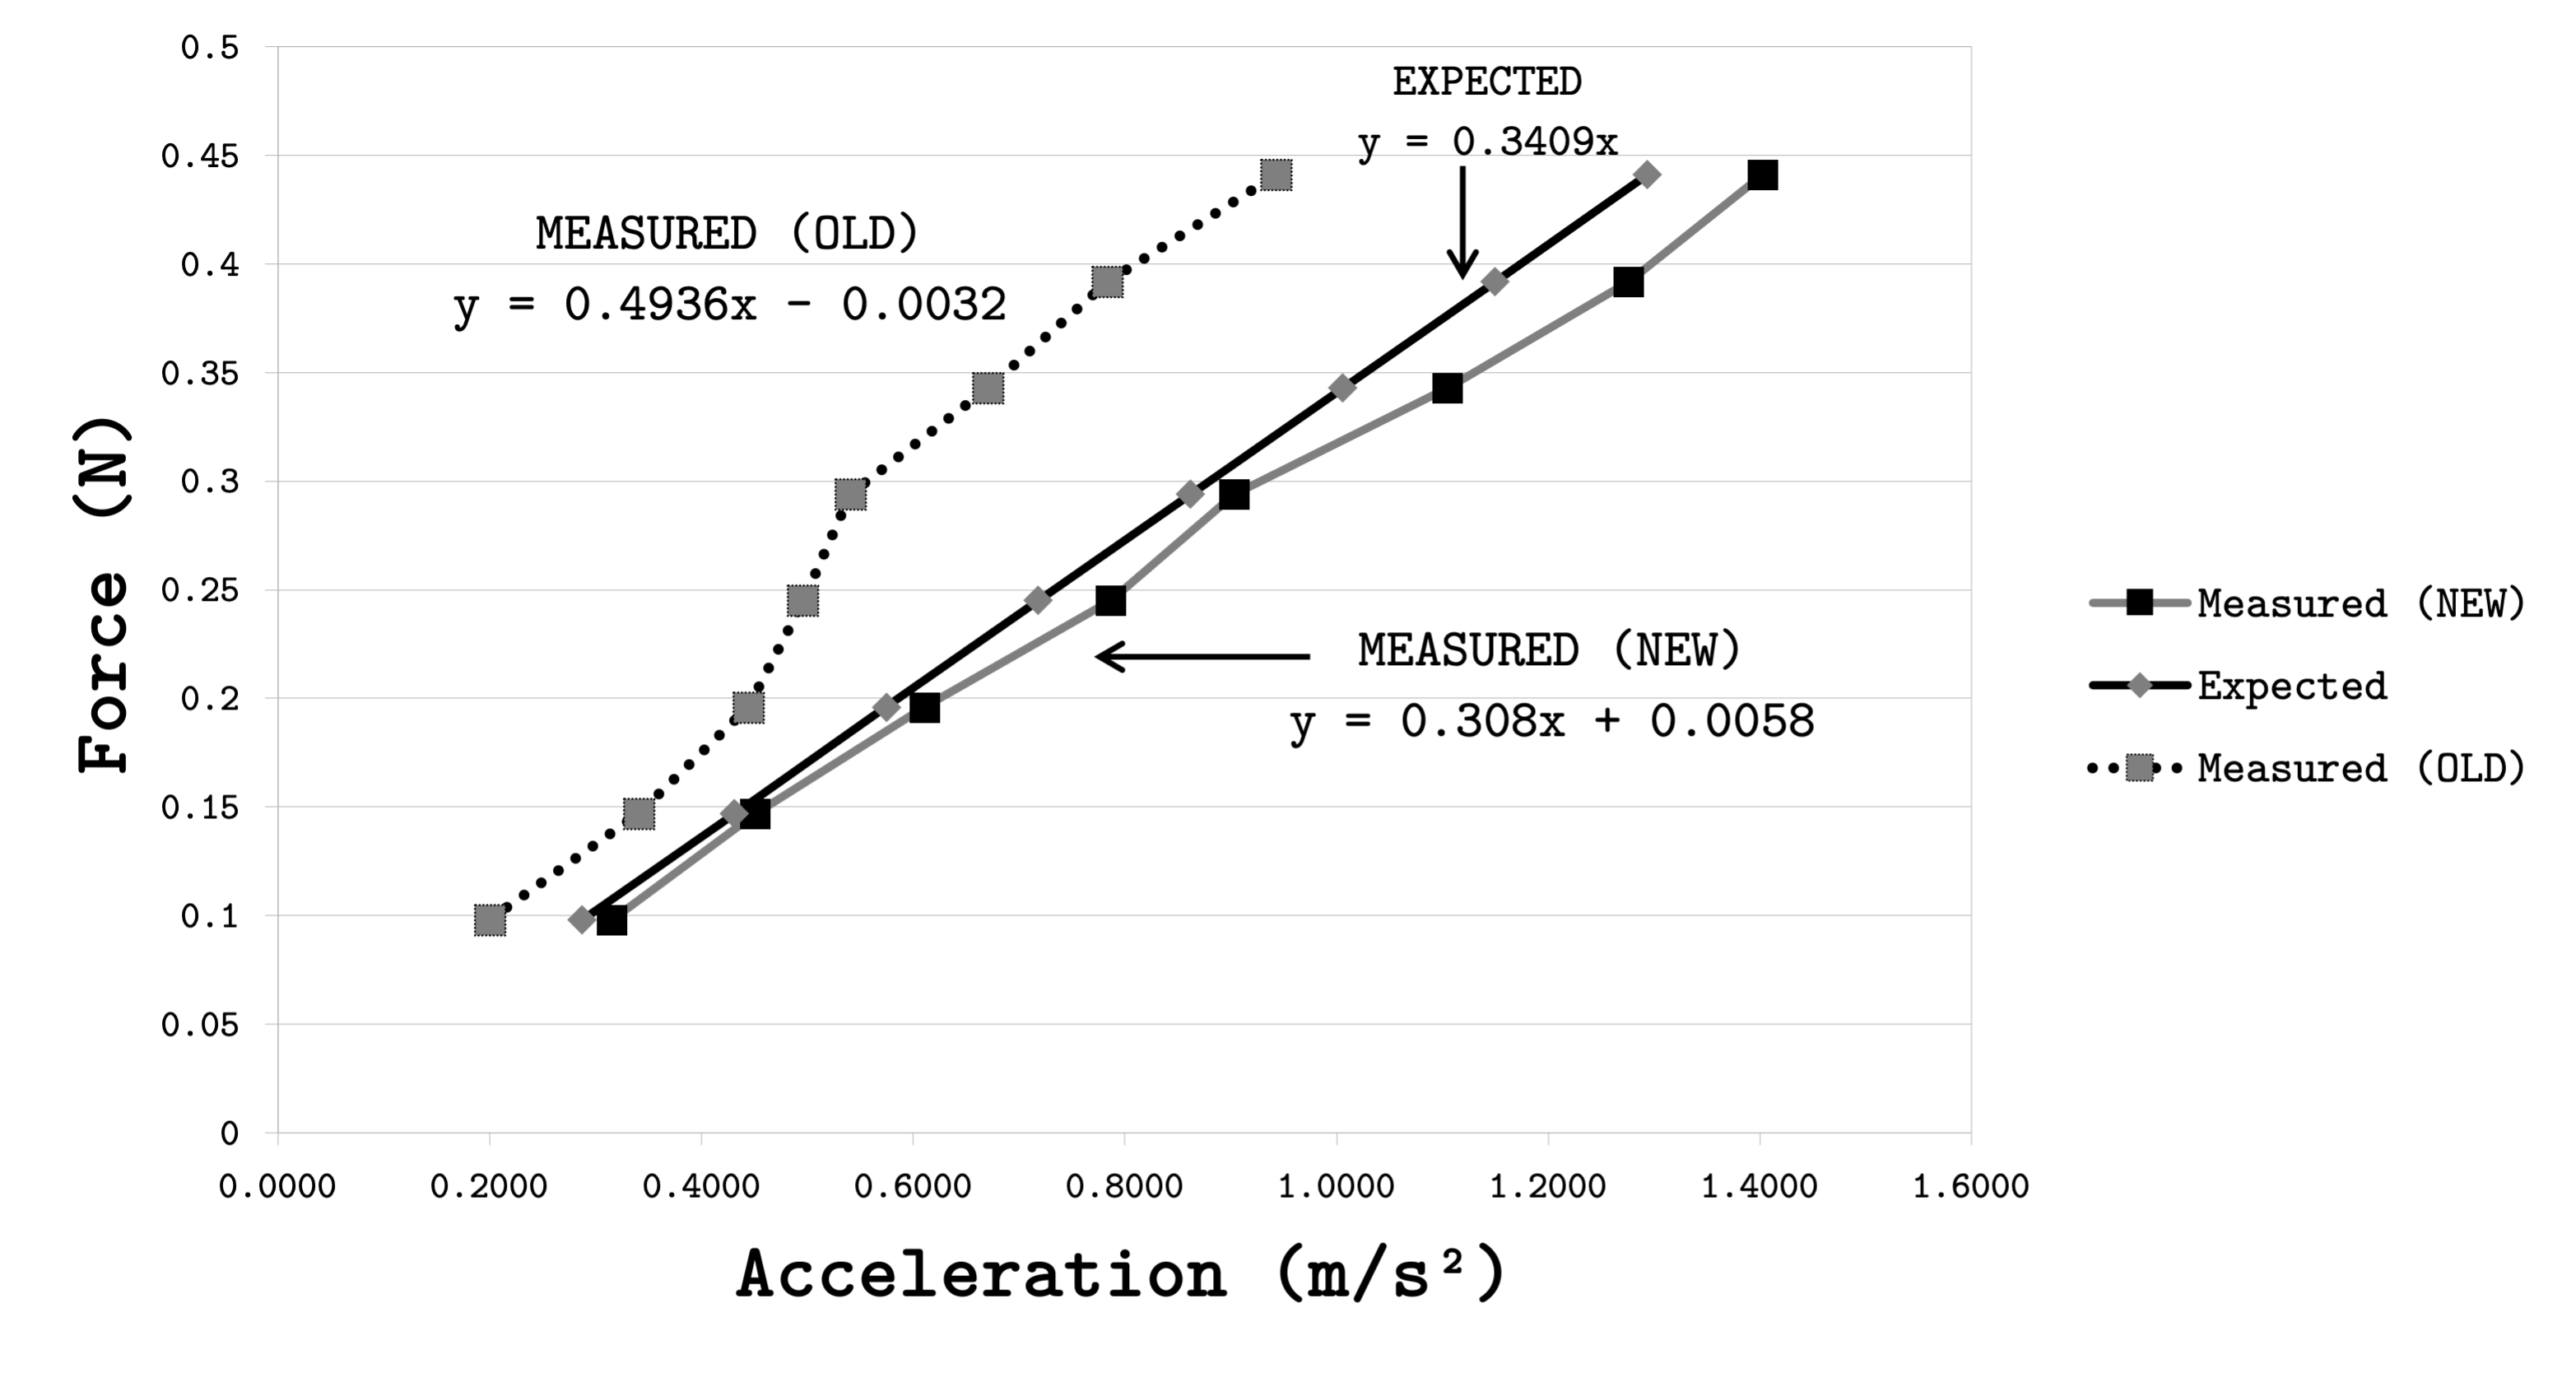
\includegraphics[width=0.90\columnwidth]{images/GraphFvA}
% 	\end{center}
% \end{figure}
% \end{landscape}

\begin{figure}[H]
	\captionsetup{font=Large}
	\caption{Part 1: Actual F\textsubscript{c} vs Actual Average Velocity}
	\begin{center}
		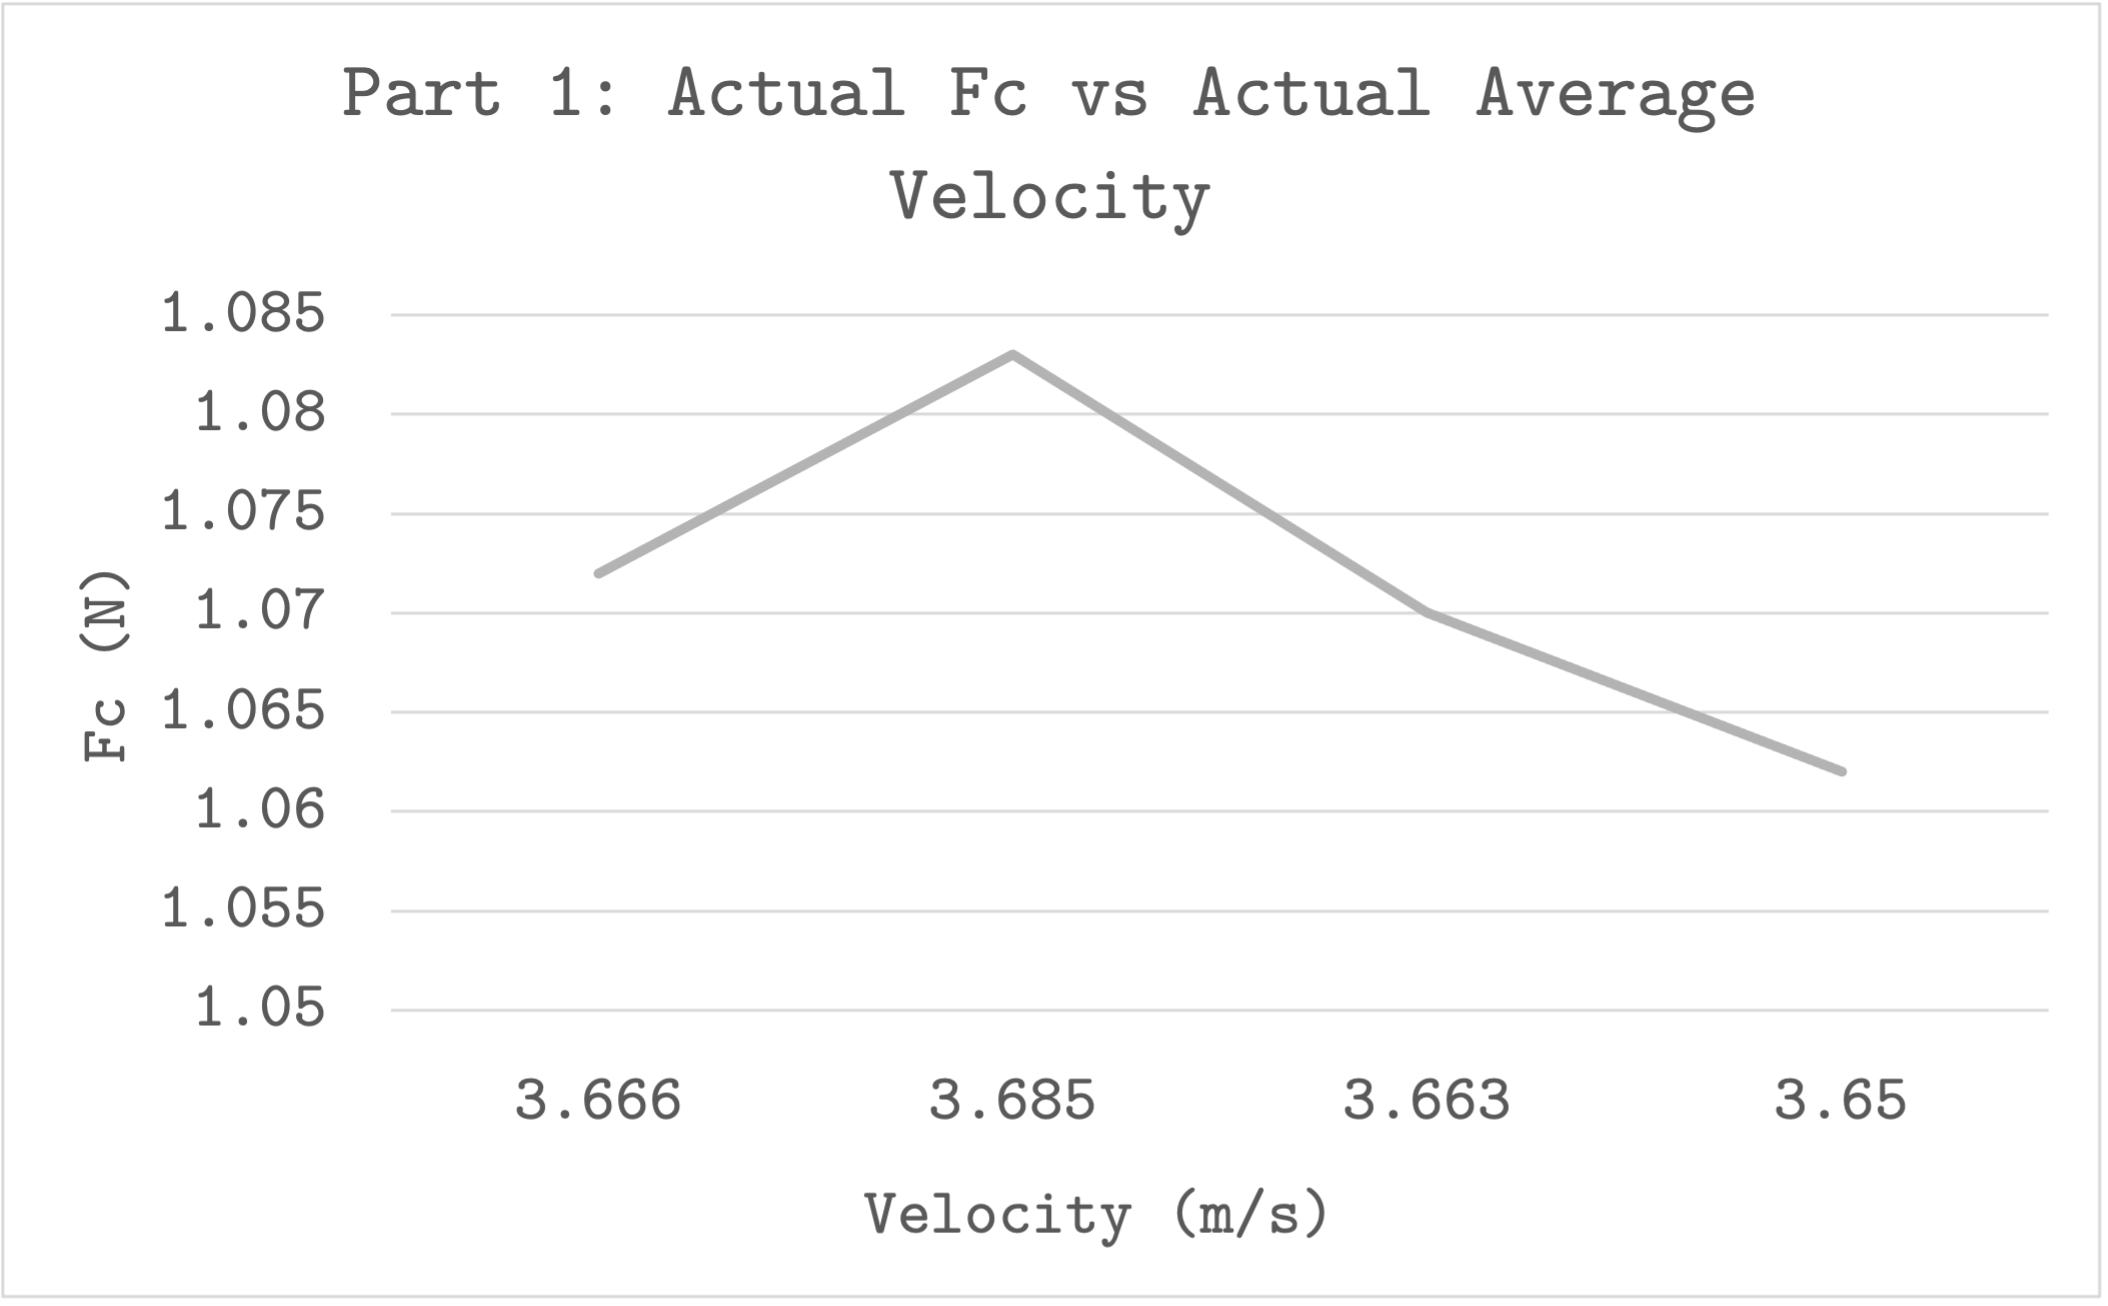
\includegraphics[width=0.90\textwidth]{images/p1Actual}
	\end{center}
	\label{fig:p1Actual}
\end{figure}

\begin{figure}[H]
	\captionsetup{font=Large}
	\caption{Part 1: Expected F\textsubscript{c} vs Expected Velocity}
	\begin{center}
		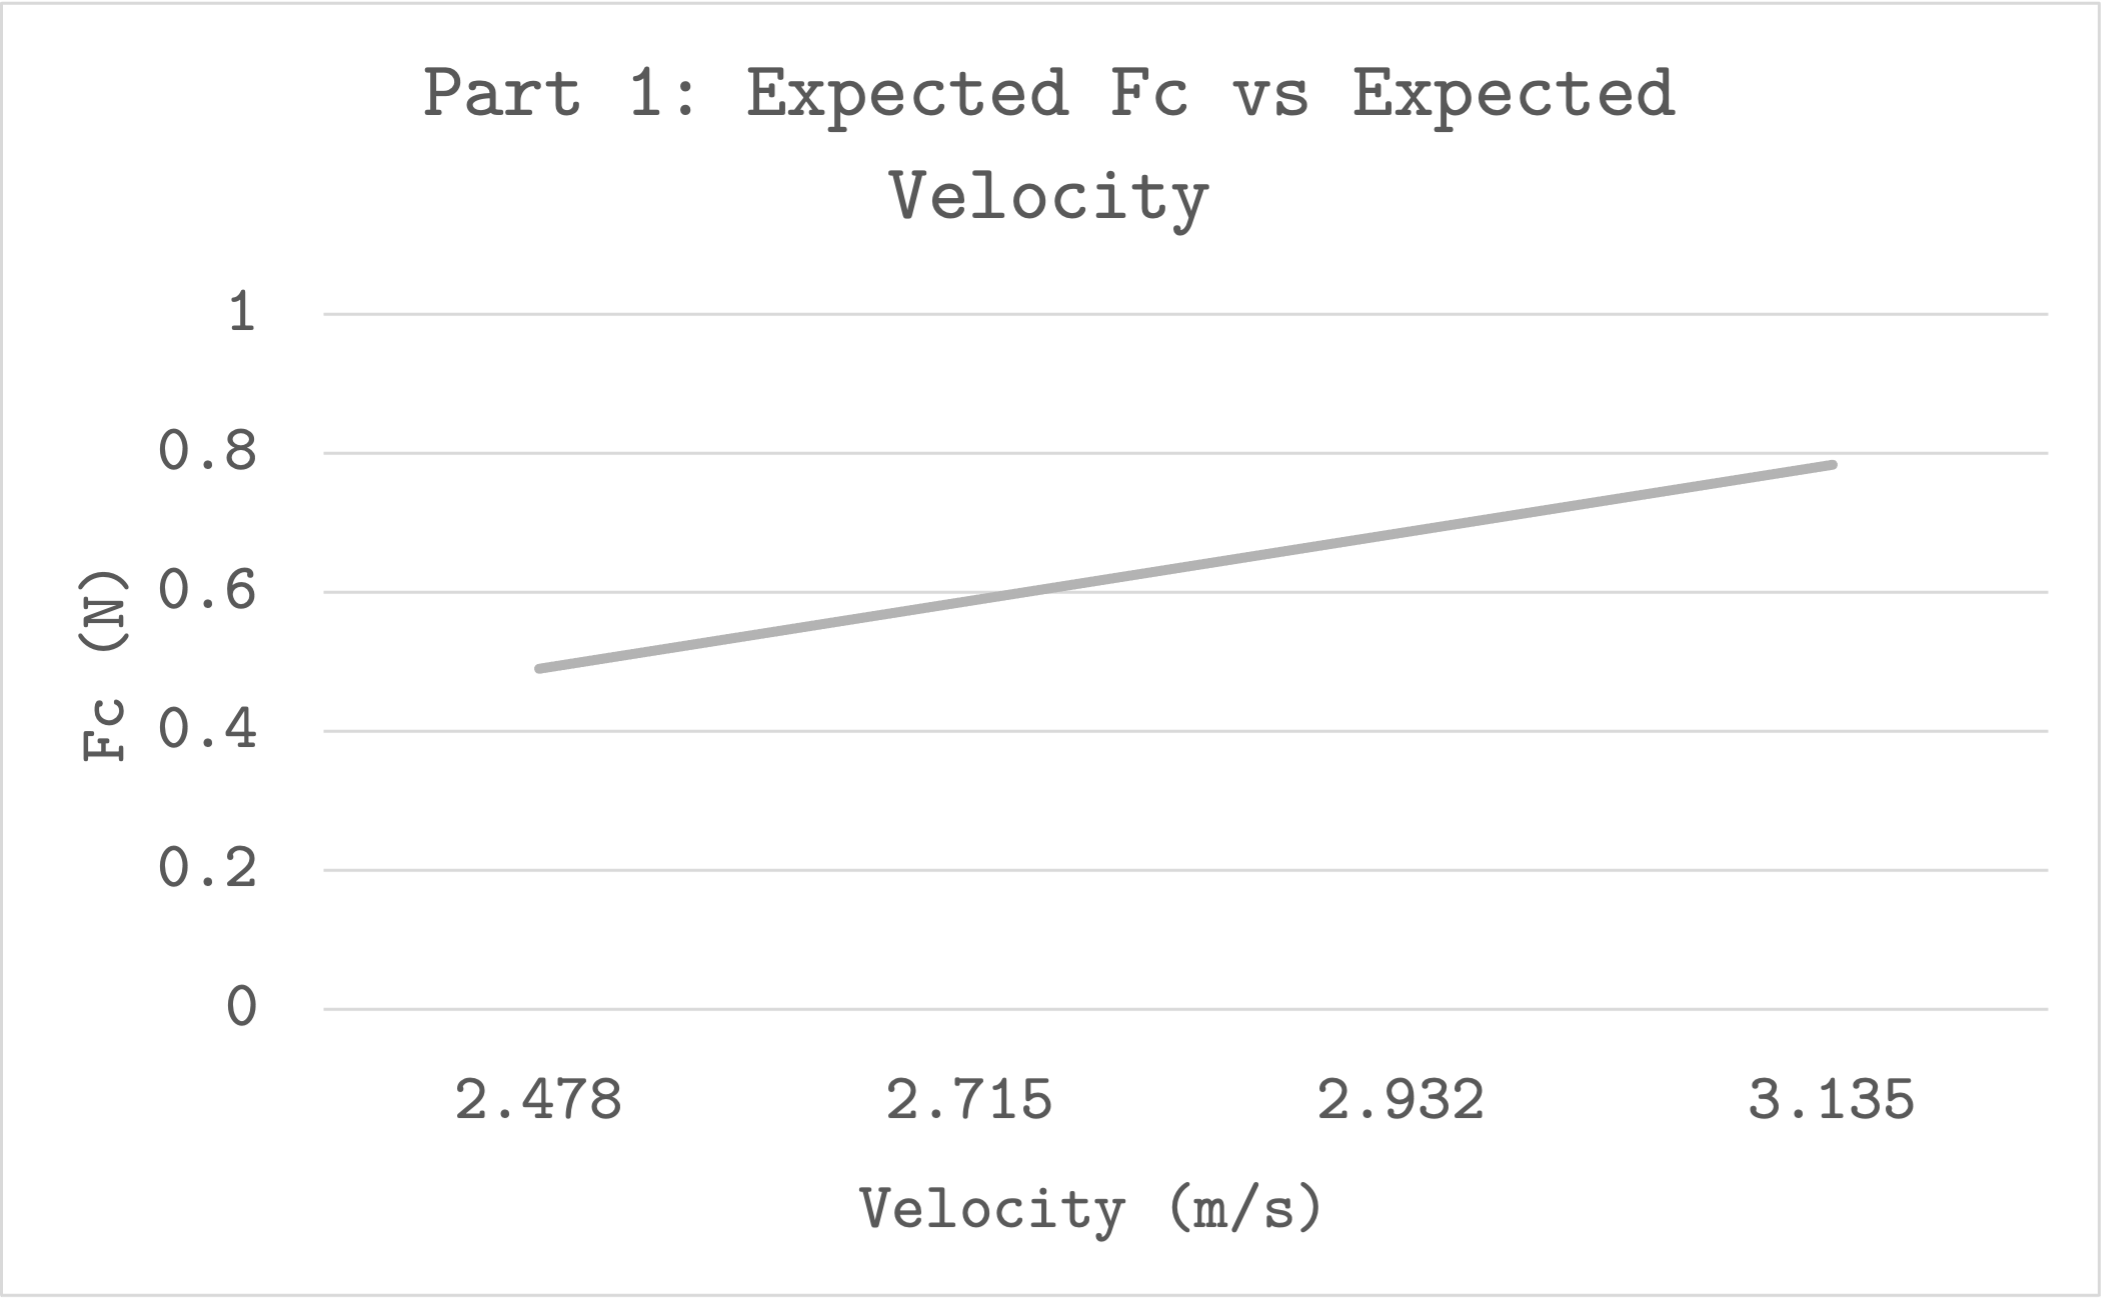
\includegraphics[width=0.90\textwidth]{images/p1Expected}
	\end{center}
	\label{fig:p1Expected}
\end{figure}


\begin{figure}[H]
	\captionsetup{font=Large}
	\caption{Part 3: Radius vs Actual Average Velocity}
	\begin{center}
		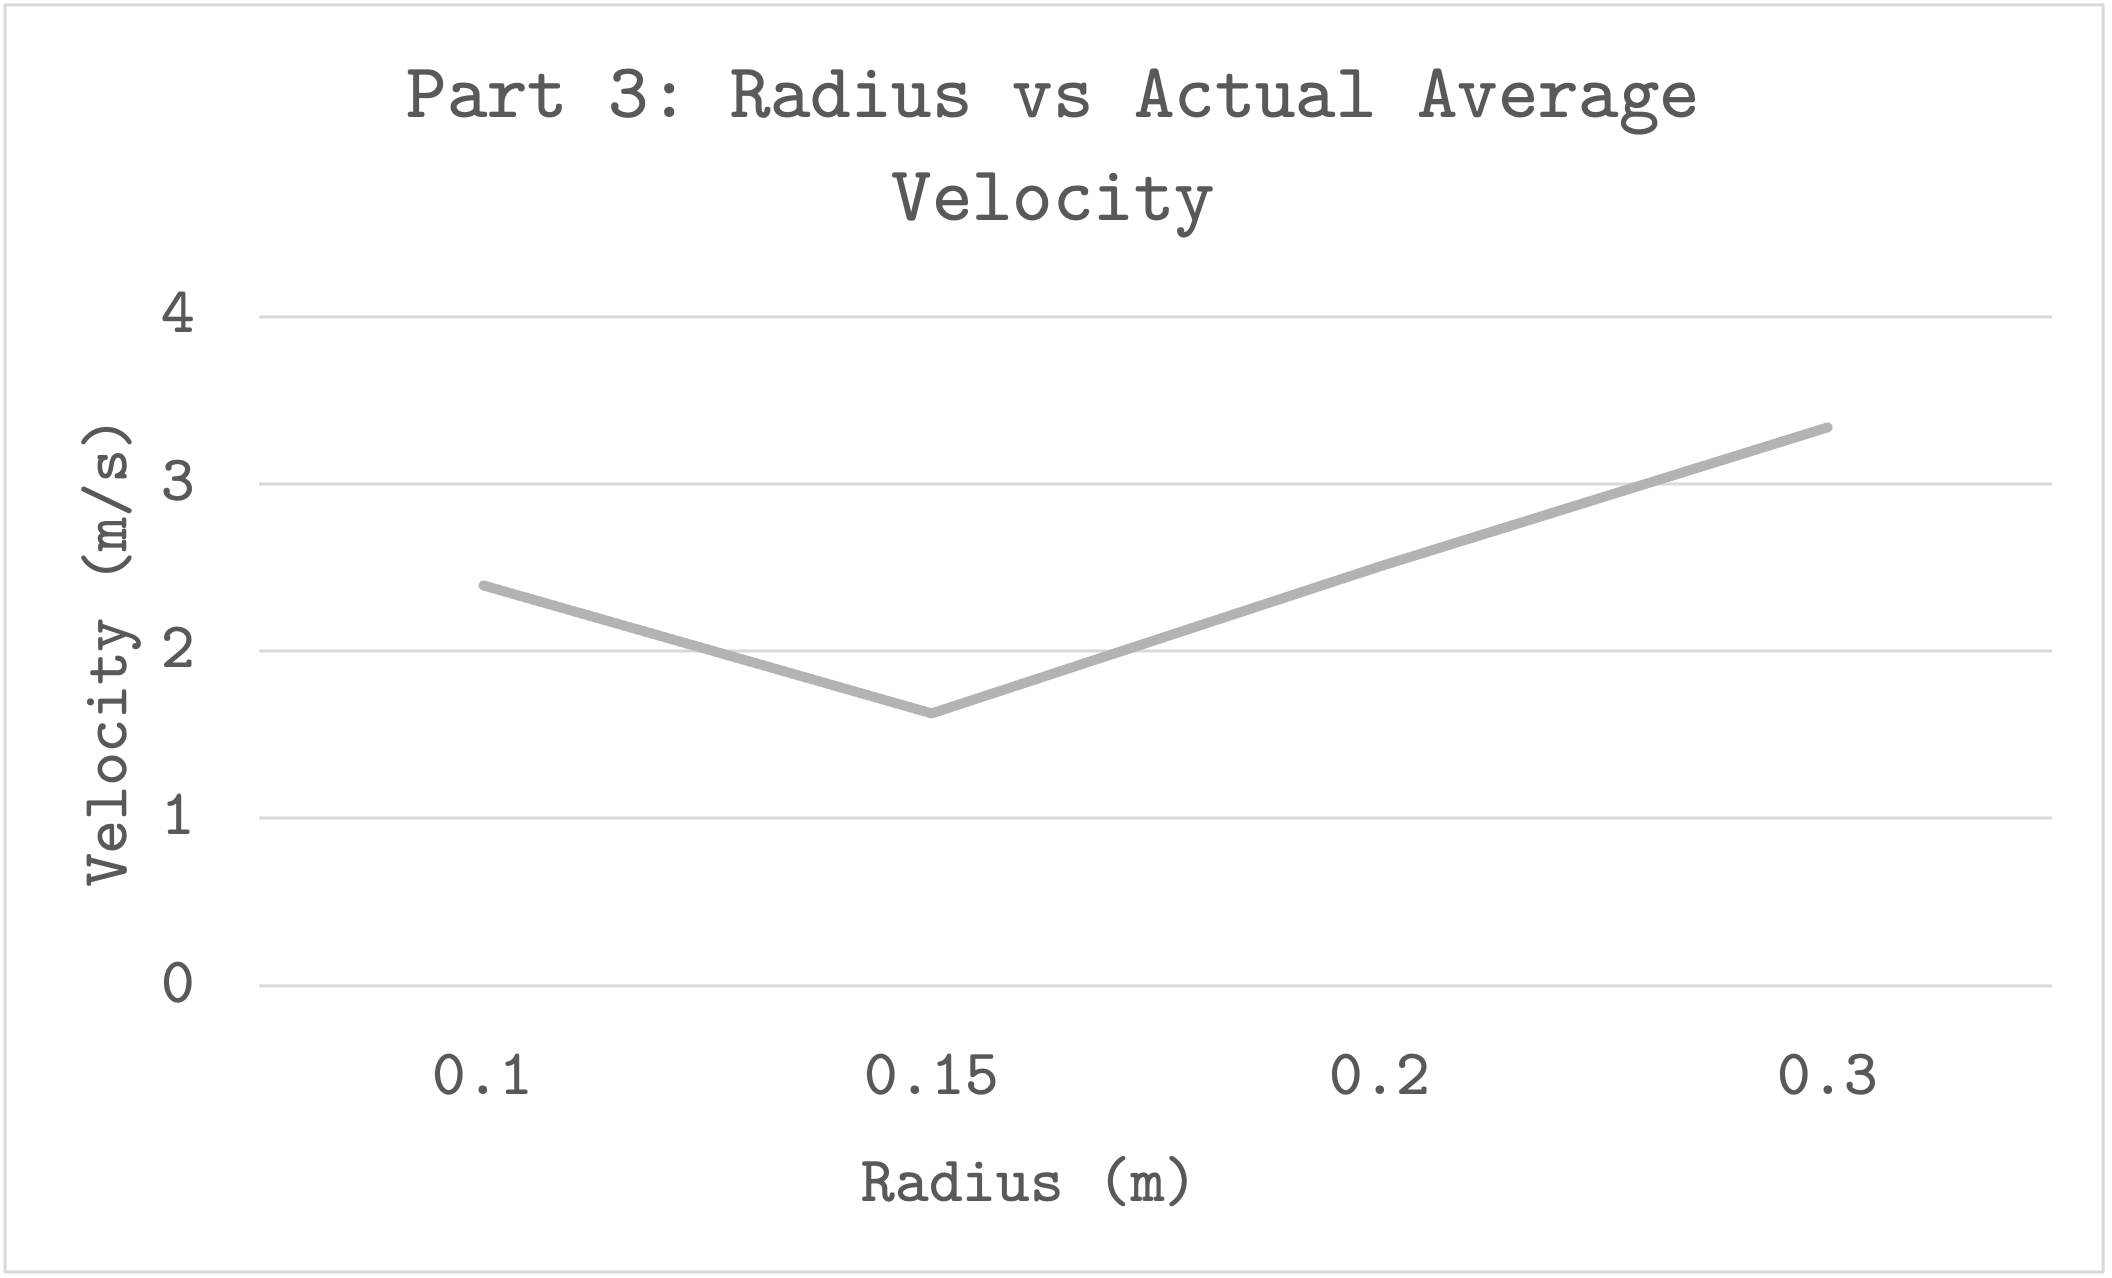
\includegraphics[width=0.90\textwidth]{images/p3Actual}
	\end{center}
	\label{fig:p3Actual}
\end{figure}

\begin{figure}[H]
	\captionsetup{font=Large}
	\caption{Part 3: Radius vs Expected Velocity}
	\begin{center}
		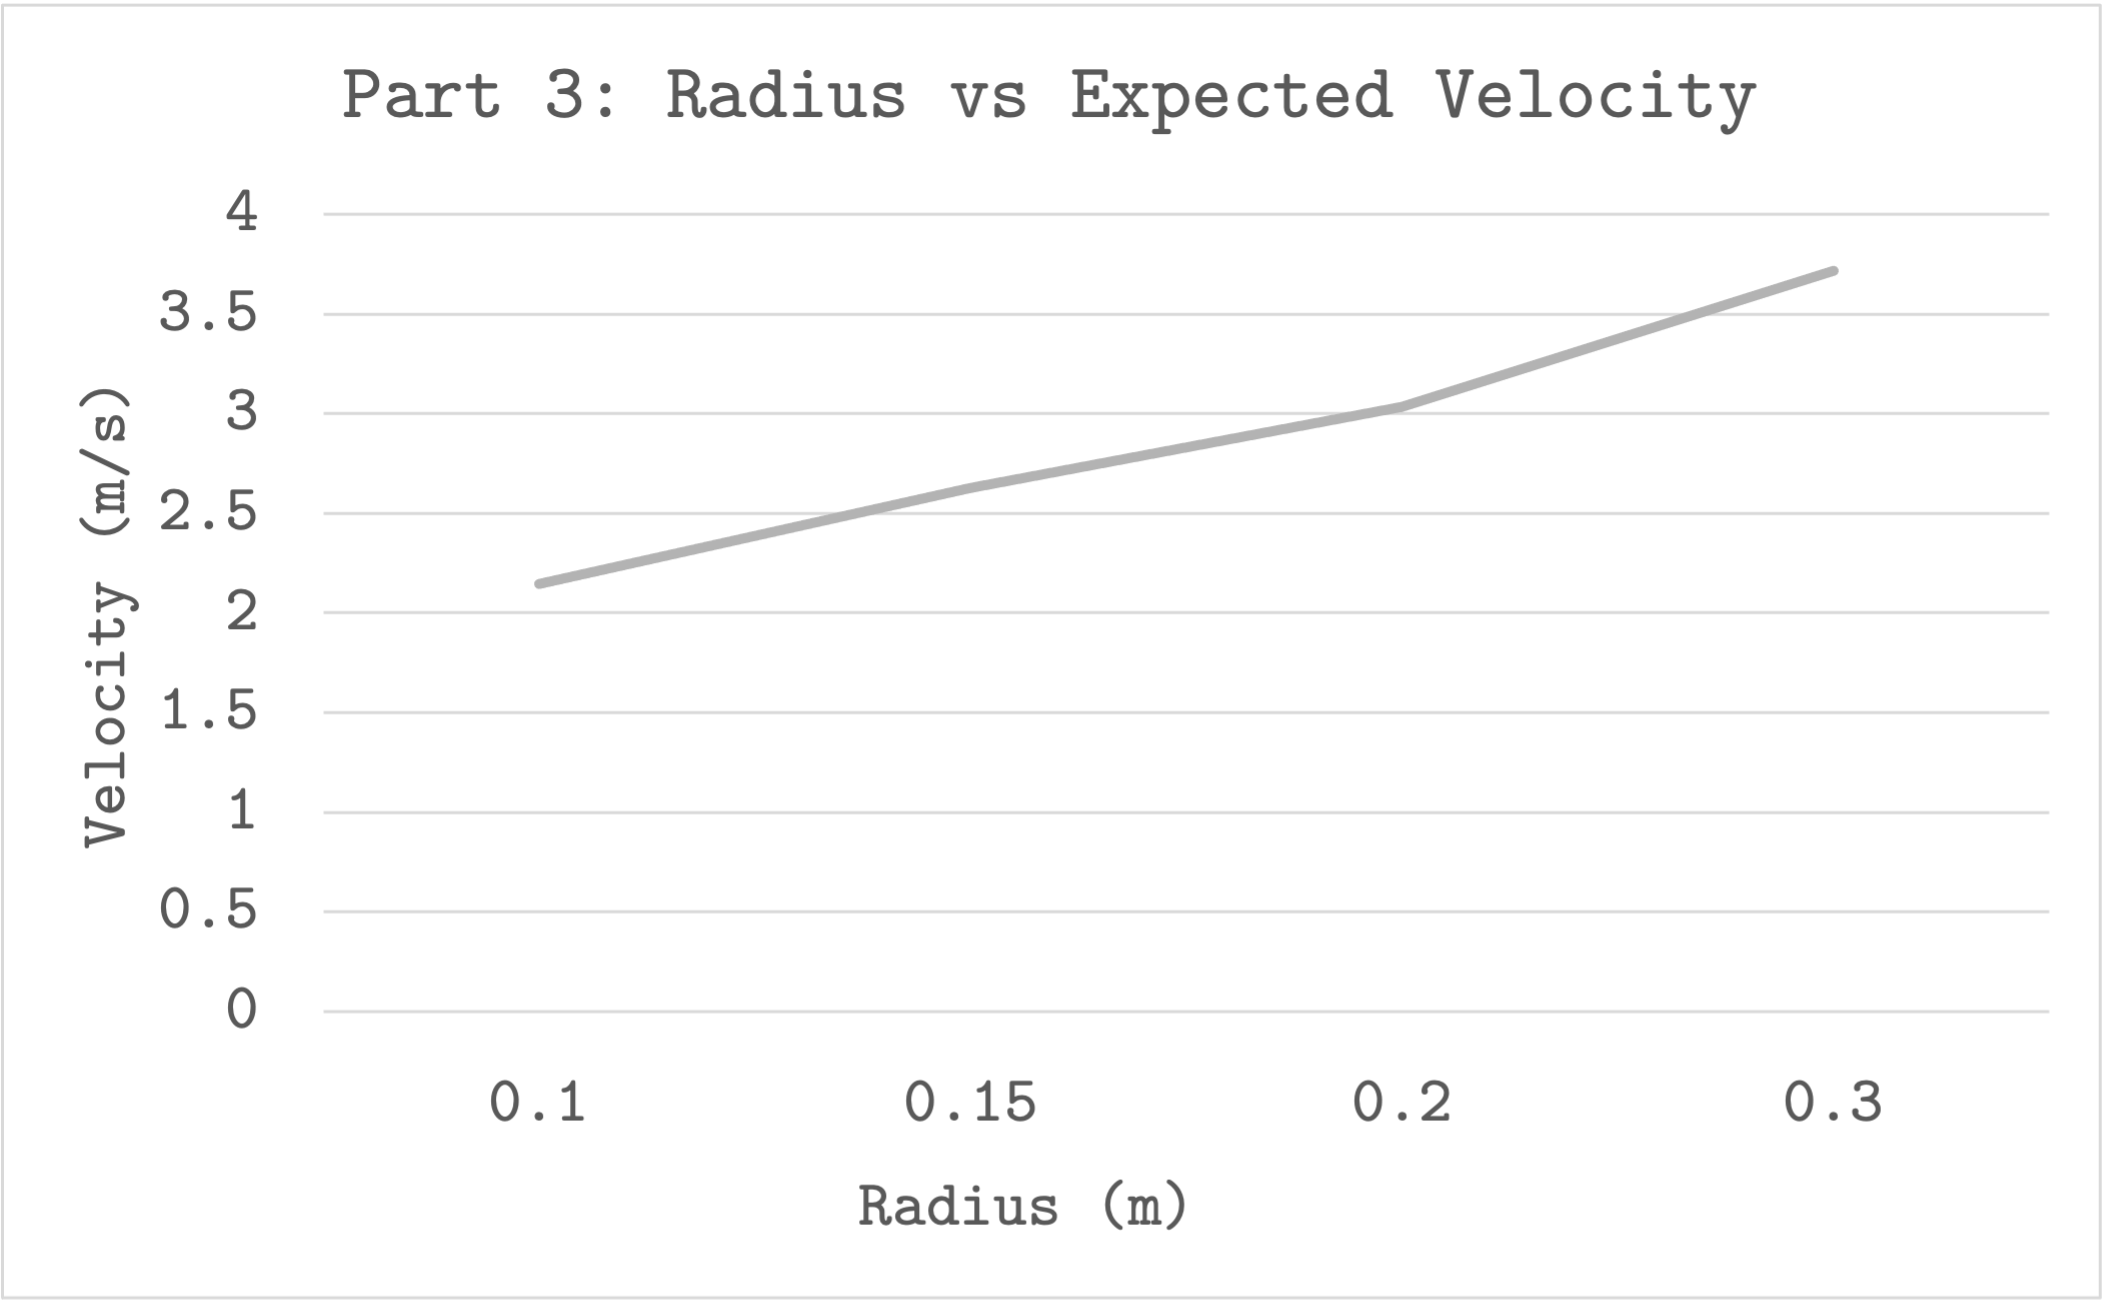
\includegraphics[width=0.90\textwidth]{images/p3Expected}
	\end{center}
	\label{fig:p3Expected}
\end{figure}

%----GRAPHS-----%

\newpage

